\documentclass[conference, onecolumn]{IEEEtran}
% \usepackage[pdftex]{graphicx}
% \usepackage[dvips]{graphicx}
%\usepackage{amsmath}
\usepackage{algorithm}
\usepackage{algorithmic}
%\usepackage{array}
%\usepackage[caption=false,font=normalsize,labelfont=sf,textfont=sf]{subfig}
%\usepackage{fixltx2e}
%\usepackage{stfloats}
%\usepackage{url}
\usepackage{amsmath}
\usepackage{amssymb}
\RequirePackage{amsfonts}
\RequirePackage{standalone}
\RequirePackage{tikz}
\usetikzlibrary{matrix,backgrounds,calc,shapes,arrows,arrows.meta,fit,positioning}                                                                
\usetikzlibrary{chains,shapes.multipart}                                                                                                          
\usetikzlibrary{shapes,calc} 

\usepackage{listings}
\usepackage{color}

\definecolor{dkgreen}{rgb}{0,0.6,0}
\definecolor{gray}{rgb}{0.5,0.5,0.5}
\definecolor{mauve}{rgb}{0.58,0,0.82}

\lstset{frame=tb,
language=C,
aboveskip=3mm,
belowskip=3mm,
showstringspaces=false,
basicstyle={\small\ttfamily},
numbers=none,
numberstyle=\tiny\color{gray},
keywordstyle=\color{blue},
commentstyle=\color{dkgreen},
stringstyle=\color{mauve},
breaklines=true,
breakatwhitespace=true,
tabsize=4
}

%columns=flexible,
\hyphenation{op-tical net-works semi-conduc-tor}


\begin{document}

\title{MicroPP: Reference Manual}

\author{\IEEEauthorblockN{
	Guido Giuntoli\IEEEauthorrefmark{1}\IEEEauthorrefmark{2},
	Jimmy Aguilar\IEEEauthorrefmark{1}\IEEEauthorrefmark{3}}
\IEEEauthorblockA{\IEEEauthorrefmark{1}Barcelona Supercomputing Center}
\IEEEauthorblockA{\IEEEauthorrefmark{2}guido.giuntoli@bsc.es}
\IEEEauthorblockA{\IEEEauthorrefmark{3}jimmy.aguilar@bsc.es}}

\maketitle

% no keywords

\IEEEpeerreviewmaketitle

\section{Introduction}
% no \IEEEPARstart

\hfill August 26, 2015

\section{Governing Equations And FE Method}

\begin{equation}
\left\{
\begin{array}{ll}
	\nabla \cdot \sigma = 0 &\;\text{ in } \;\Omega,\\
	u = \overline{\epsilon} \cdot x &\;\text{ in } \;x \in \Gamma,\\
	\sigma = f(\epsilon,q).
\end{array}
\right.
\label{eq:micro}
\end{equation}


\section{Implementation}

\begin{figure}[!hhh]
	\centering
	\resizebox{5cm}{!}{\documentclass{standalone}

\begin{document}

\tikzset{cross/.style={cross out, draw=black, fill=none, minimum size=2*(#1-\pgflinewidth), inner sep=0pt, outer sep=0pt}, cross/.default={2pt}}

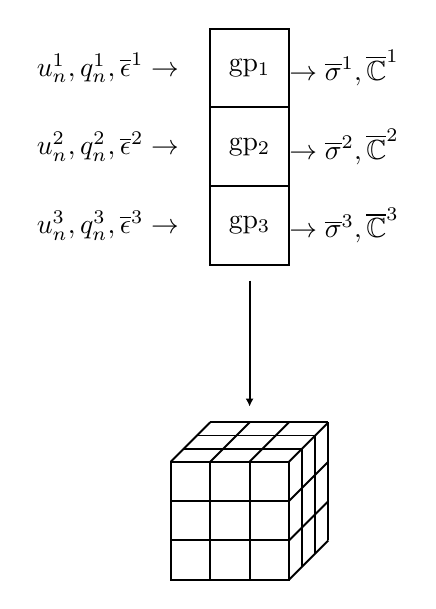
\begin{tikzpicture}[>=latex,node distance=0pt, line width=0.25mm]

   \draw [black] (0,0) -- (1,0) -- (1,3) -- (0,3) -- cycle;
   \draw [black] (0,1) -- (1,1);
   \draw [black] (0,2) -- (1,2);
   \node[draw=none,scale=1.0] at (0.5,0.5) {gp$_3$};
   \node[draw=none,scale=1.0] at (0.5,1.5) {gp$_2$};
   \node[draw=none,scale=1.0] at (0.5,2.5) {gp$_1$};

   \node[draw=none,scale=1.0] at (-1.3,0.5) {$u_n^3,q_n^3,\overline{\epsilon}^3 \rightarrow$};
   \node[draw=none,scale=1.0] at (-1.3,1.5) {$u_n^2,q_n^2,\overline{\epsilon}^2 \rightarrow$};
   \node[draw=none,scale=1.0] at (-1.3,2.5) {$u_n^1,q_n^1,\overline{\epsilon}^1 \rightarrow$};
   \node[draw=none,scale=1.0] at (1.7,0.5) {$\rightarrow \overline{\sigma}^3, \overline{\mathbb{C}}^3$};
   \node[draw=none,scale=1.0] at (1.7,1.5) {$\rightarrow \overline{\sigma}^2, \overline{\mathbb{C}}^2$};
   \node[draw=none,scale=1.0] at (1.7,2.5) {$\rightarrow \overline{\sigma}^1, \overline{\mathbb{C}}^1$};

   \draw[-{Latex[length=1mm,width=1mm]}] (0.5,-.2) -- ++(0,-1.6);

   \begin{scope}[xshift=-0.5cm,yshift=-4cm,scale=0.5]
      \draw [black] (0,0) -- (3,0) -- (3,3) -- (0,3) -- cycle;
      \draw [black] (0,3) -- ++(1,1);
      \draw [black] (3,3) -- ++(1,1);
      \draw [black] (3,0) -- ++(1,1);
      \draw [black] (4,1) -- ++(0,3);
      \draw [black] (1,4) -- ++(3,0);
      \draw [black] (0,1) -- ++(3,0);
      \draw [black] (0,2) -- ++(3,0);
      \draw [black] (1,0) -- ++(0,3);
      \draw [black] (2,0) -- ++(0,3);
      \draw [black] (1,3) -- ++(1,1);
      \draw [black] (2,3) -- ++(1,1);
      \draw [black] (3,1) -- ++(1,1);
      \draw [black] (3,2) -- ++(1,1);
      \draw [black] (0.333,3.333) -- ++(3,0);
      \draw [black] (0.666,3.666) -- ++(3,0);
      \draw [black] (3.333,0.333) -- ++(0,3);
      \draw [black] (3.666,0.666) -- ++(0,3);
   \end{scope}

\end{tikzpicture}
\end{document}
}
	\vspace{0.5cm}
	\caption{\label{fig:comp_scheme}}
\end{figure}

The Voigt convention used here is the same as in Ref.~\cite{simo}.
\begin{equation}
\epsilon = \left[\epsilon_{11} \quad \epsilon_{22} \quad \epsilon_{33} \quad \epsilon_{12} \quad \epsilon_{13} \quad \epsilon_{23} \right]^T
\end{equation}

\section{Geometries}

\section{Material Models}

\subsubsection{Plasticity Model}

MicroPP has a J2 plasticity model with isotropic hardening.

\begin {equation}
\left\{
\begin{array}{ll}
\epsilon_{n+1}^{e,\text{trial}} = \epsilon_{n+1} - \epsilon_{n}^{p} \\[5pt]
\sigma_{n+1}^{\text{trial}} = \mathrm{C} : \epsilon_{n+1}^{e,\text{trial}} \\[5pt]
\mathbf{q}_{n+1}^{\text{trial}} = \mathbf{q}_{n} \\[5pt]
f_{n+1}^{\text{trial}} = f (\sigma_{n+1}^{\text{trial}}, \mathbf{q}_{n+1}^{\text{trial}})\\
\end{array}
\right.
\end {equation}

\begin {equation}
\left\{
\begin{array}{ll}
\epsilon_{n+1}^{p} = \epsilon_{n}^{p} - \Delta \gamma  \mathbf{n}_{n+1} \\[5pt]
\alpha_{n+1} = \alpha_{n} + \sqrt{\frac{2}{3}} \Delta \gamma
\end{array}
\right.
\end {equation}

\begin {equation}
s_{n+1}^{\text{trial}} = s_{n+1} + 2 \mu e_{n+1}
\end {equation}

\begin {equation}
\mathbf{n}_{n+1} = \frac{s_{n+1}^{\text{trial}}}{|| s_{n+1}^{\text{trial}} ||}
\end {equation}

\begin {equation}
f_{n+1}^{\text{trial}} = || s_{n+1}^{\text{trial}} || - \sqrt{\frac{2}{3}} (\sigma_{Y} + K_{a} \alpha_{n} )
\end {equation}

\begin {equation}
\Delta \gamma = \frac{f_{n+1}^{\text{trial}}}{2\mu(1+K_{a})}
\end {equation}

1. Compute trial elastic stress
\begin {equation}
\left\{
\begin{array}{ll}
e_{n+1} = \epsilon_{n+1} - \frac{1}{3} \text{tr}( \epsilon_{n+1} ) \\[5pt]
s_{n+1}^{\text{trial}} = 2\mu( e_{n+1} - e_{n+1}^{p} ) \\[5pt]
\end{array}
\right.
\end {equation}

2. Check yield condition

\begin {equation}
f_{n+1}^{\text{trial}} = || s_{n+1}^{\text{trial}} || - \sqrt{\frac{2}{3}} (\sigma_{Y} + K_{a} \alpha_{n} )
\end {equation}

3. If $f_{n+1}^{\text{trial}} < 0$ then set
\begin {equation}
(\cdot)_{n+1} = (\cdot)_{n+1}^{\text{trial}} \text{ and exit.}
\end {equation}

\begin {equation}
\Delta \gamma = \frac{f_{n+1}^{\text{trial}}}{2\mu(1+K_{a})}
\end {equation}

4. Compute
\begin {equation}
\mathbf{n}_{n+1} = \frac{s_{n+1}^{\text{trial}}}{|| s_{n+1}^{\text{trial}} ||}
\end {equation}

\begin {equation}
\Delta \gamma = \frac{f_{n+1}^{\text{trial}}}{2\mu(1+K_{a})}
\end {equation}

5. Update variables
\begin {equation}
\left\{
\begin{array}{ll}
\epsilon_{n+1}^{p} = \epsilon_{n}^{p} - \Delta \gamma  \mathbf{n}_{n+1} \\[5pt]
\alpha_{n+1} = \alpha_{n} + \sqrt{\frac{2}{3}} \Delta \gamma \\[5pt]
\sigma_{n+1} = k \, \text{tr} (\epsilon_{n+1}) + s_{n+1}^{\text{trial}} - 2 \mu \Delta \gamma \mathbf{n}_{n+1} 
\end{array}
\right.
\end {equation}

\begin{algorithm}
\caption{Algorithm caption}
\label{alg:algorithm-label}
\begin{algorithmic}
 \STATE $ \epsilon^{0} = \epsilon $
 \STATE $ \sigma^{0} = g(\epsilon^{0})$
 \FOR {$i=1\dots6$}
     \STATE $ \epsilon^{*} = \epsilon $
     \STATE $ \epsilon^{*}(i) = \epsilon^{*}(i) + \delta\epsilon $
     \STATE $ \sigma^{*} = g(\epsilon^{*})$
     \STATE $ \mathrm{C} (i, :) = ( \sigma^* - \sigma^0 ) / \delta\epsilon $
 \ENDFOR
\end{algorithmic}
\end{algorithm}

\section{Coding Style}

The coding style should be follow in all .cpp, .hpp, and .f95 files that are present in the code.

\subsection{License}

All source files should have the GPL License header with the corresponding contributors.

\begin{lstlisting}

/*
 *  This source code is part of MicroPP: a finite element library
 *  to solve microstructural problems for composite materials.
 *
 *  Copyright (C) - 2018 - Jimmy Aguilar Mena <kratsbinovish@gmail.com>
 *                         Guido Giuntoli <gagiuntoli@gmail.com>
 *
 *  This program is free software: you can redistribute it and/or modify
 *  it under the terms of the GNU General Public License as published by
 *  the Free Software Foundation, either version 3 of the License, or
 *  (at your option) any later version.
 *
 *  This program is distributed in the hope that it will be useful,
 *  but WITHOUT ANY WARRANTY; without even the implied warranty of
 *  MERCHANTABILITY or FITNESS FOR A PARTICULAR PURPOSE.  See the
 *  GNU General Public License for more details.
 *
 *  You should have received a copy of the GNU General Public License
 *  along with this program.  If not, see <https://www.gnu.org/licenses/>.
 */

\end{lstlisting}

\subsection{Functions Definitions}

Most of the functions in the code are templates. This was done to separate 2D from 3D cases and to produce a more readable code. Functions' arguments can have the \verb const at the beginning but we don't we try to not use it in does cases where it is obvious that the two arguments are not going to be modified. In some cases it it useful if it is applied to pointers like {\verb#int const * a#}.

\begin{lstlisting}

template <int tdim>
int micropp<tdim>::calc_average(const int gp,
                                 double * array
				 int n)
{
	INST_START; /* This is to instrument this function */

	int average = gp + 2.3 / 9.;
	for(int i = 0; i < n / 2; ++i)
		array[i] = average;
	return average;
}
\end{lstlisting}

\subsection{Control Flow Statements}


The \verb if  statements should be written:

\begin{lstlisting}

if(a == 3 && b < 4.) {
    calc_average(a, array, n);
} else if(k % 3 = 2) {
    calc_average(c, array, n);
}

if(calc_average(c, array, n))
    exit(0);

\end{lstlisting}

The \verb for  statements should be written:

\begin{lstlisting}

for(int i = 0; i < n; ++i) {
    a += array[i] + 9.4;
}

for(int i = 0; i < n; ++i)
    for(int j = 0; j < n; ++j)
        array[i * n + j] = A[i][j];

\end{lstlisting}


\section{Conclusion}
The conclusion goes here.

% use section* for acknowledgment
\section*{Acknowledgment}

The authors would like to thank...

\begin{thebibliography}{1}
\bibitem{simo} J.C. Simo \& T.J.R. Huges.\emph{Computational Ineslasticity}, Springer, 2000. 
\bibitem{oller} S. Oller. \emph{Numerical Simulation of Mechanical Behavior of Composite Materials}, Springer, 2014. 
\end{thebibliography}

\end{document}
